% Options for packages loaded elsewhere
\PassOptionsToPackage{unicode}{hyperref}
\PassOptionsToPackage{hyphens}{url}
%
\documentclass[
]{book}
\usepackage{lmodern}
\usepackage{amssymb,amsmath}
\usepackage{ifxetex,ifluatex}
\ifnum 0\ifxetex 1\fi\ifluatex 1\fi=0 % if pdftex
  \usepackage[T1]{fontenc}
  \usepackage[utf8]{inputenc}
  \usepackage{textcomp} % provide euro and other symbols
\else % if luatex or xetex
  \usepackage{unicode-math}
  \defaultfontfeatures{Scale=MatchLowercase}
  \defaultfontfeatures[\rmfamily]{Ligatures=TeX,Scale=1}
\fi
% Use upquote if available, for straight quotes in verbatim environments
\IfFileExists{upquote.sty}{\usepackage{upquote}}{}
\IfFileExists{microtype.sty}{% use microtype if available
  \usepackage[]{microtype}
  \UseMicrotypeSet[protrusion]{basicmath} % disable protrusion for tt fonts
}{}
\makeatletter
\@ifundefined{KOMAClassName}{% if non-KOMA class
  \IfFileExists{parskip.sty}{%
    \usepackage{parskip}
  }{% else
    \setlength{\parindent}{0pt}
    \setlength{\parskip}{6pt plus 2pt minus 1pt}}
}{% if KOMA class
  \KOMAoptions{parskip=half}}
\makeatother
\usepackage{xcolor}
\IfFileExists{xurl.sty}{\usepackage{xurl}}{} % add URL line breaks if available
\IfFileExists{bookmark.sty}{\usepackage{bookmark}}{\usepackage{hyperref}}
\hypersetup{
  pdftitle={Software Installation Guide},
  pdfauthor={Francisco Rowe, Dani Arribas-Bel},
  hidelinks,
  pdfcreator={LaTeX via pandoc}}
\urlstyle{same} % disable monospaced font for URLs
\usepackage{longtable,booktabs}
% Correct order of tables after \paragraph or \subparagraph
\usepackage{etoolbox}
\makeatletter
\patchcmd\longtable{\par}{\if@noskipsec\mbox{}\fi\par}{}{}
\makeatother
% Allow footnotes in longtable head/foot
\IfFileExists{footnotehyper.sty}{\usepackage{footnotehyper}}{\usepackage{footnote}}
\makesavenoteenv{longtable}
\usepackage{graphicx,grffile}
\makeatletter
\def\maxwidth{\ifdim\Gin@nat@width>\linewidth\linewidth\else\Gin@nat@width\fi}
\def\maxheight{\ifdim\Gin@nat@height>\textheight\textheight\else\Gin@nat@height\fi}
\makeatother
% Scale images if necessary, so that they will not overflow the page
% margins by default, and it is still possible to overwrite the defaults
% using explicit options in \includegraphics[width, height, ...]{}
\setkeys{Gin}{width=\maxwidth,height=\maxheight,keepaspectratio}
% Set default figure placement to htbp
\makeatletter
\def\fps@figure{htbp}
\makeatother
\setlength{\emergencystretch}{3em} % prevent overfull lines
\providecommand{\tightlist}{%
  \setlength{\itemsep}{0pt}\setlength{\parskip}{0pt}}
\setcounter{secnumdepth}{5}
\usepackage{booktabs}
\usepackage{amsthm}
\makeatletter
\def\thm@space@setup{%
  \thm@preskip=8pt plus 2pt minus 4pt
  \thm@postskip=\thm@preskip
}
\makeatother
\usepackage[]{natbib}
\bibliographystyle{apalike}

\title{Software Installation Guide}
\author{Francisco Rowe, Dani Arribas-Bel}
\date{2020-09-08}

\begin{document}
\maketitle

{
\setcounter{tocdepth}{1}
\tableofcontents
}
\hypertarget{introduction}{%
\chapter{Introduction}\label{introduction}}

\begin{itemize}
\item
  Add some brief context on why this is important and needed in the context of COVID-19 and done in Foundation Week!

  \begin{quote}
  Restricted access to University computers
  \end{quote}

  \begin{quote}
  Consistency in installation
  \end{quote}

  \begin{quote}
  No concerns with software and focus on module content during the semester
  \end{quote}
\end{itemize}

\hypertarget{purpose}{%
\section{Purpose}\label{purpose}}

This guide provides step-by-step description on how to install and access Python from your own computer. Three alternatives are described: (1) local installation via \emph{Docker}; (2) native local installation; and, (3) remote access.

\hypertarget{installation-options}{%
\section{Installation Options}\label{installation-options}}

Installation options depend on your operating system. This guide supports \textbf{MacOS}, \textbf{Linux} and \textbf{Windows} operating systems.

\hypertarget{macos-linux-and-windows-10-prostudent-users}{%
\subsection{MacOS, Linux and Windows 10 Pro/Student users}\label{macos-linux-and-windows-10-prostudent-users}}

Figure \ref{fig:fig1} displays the installation options available for \emph{MacOS}, \emph{Linux} and \emph{Windows 10 Pro/Student} users. The tree reflects our recommended installation. We strongly (1) local installation via \emph{Docker} as the default option. If that is not possible, we recommend (2) native local installation as a second option. Failing this, we recommend (3) remote access to University computers. This last option requires good and stable internet connection. If any of these options work, you must attend one of the drop-in sessions in \textbf{Foundation Week}.

\begin{figure}

{\centering 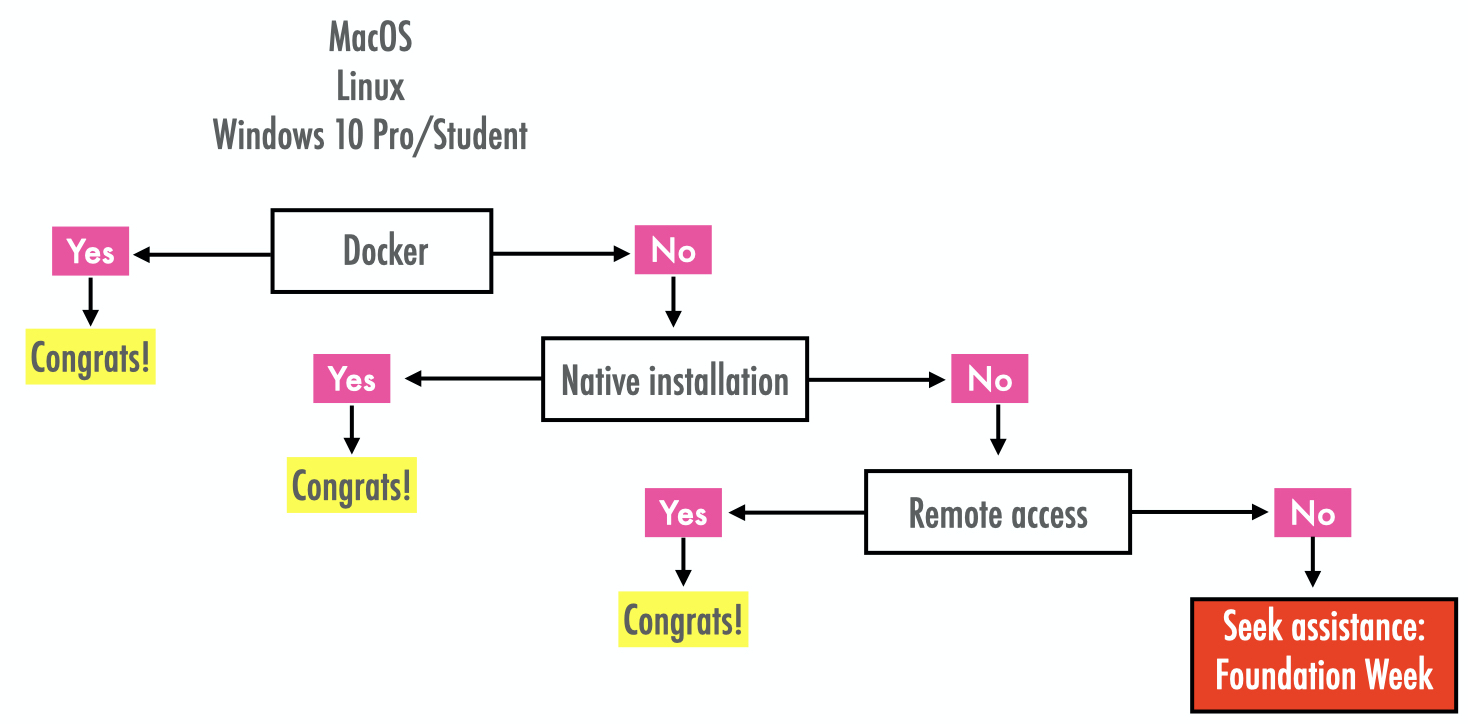
\includegraphics[width=20.39in]{figs/mac_linux_win10} 

}

\caption{Decision Tree: Recommended installation for MacOS, Linux and Windows 10 Pro/Student users}\label{fig:fig1}
\end{figure}

For step-by-step instructions of the installation options listed in Figure \ref{fig:fig1}, dedicated guides have been created. \emph{MacOS} users should refer to Chapter \ref{mac}. \emph{Linux} users should refer to Chapter @ref\{\#linux\}. \emph{Windows 10 Pro/Student} users should refer to Chapter @ref\{\#win10pro\}.

\hypertarget{other-windows-users}{%
\subsection{Other Windows users}\label{other-windows-users}}

For \textbf{other Windows users}, including other versions of Windows 10, option (1) local installation via \emph{Docker} is NOT available. Figure \ref{fig:fig2} shows the options available to these users. We strongly (1) a native local installation as the default option. If that is not possible, we recommend (2) remote access as a second option to University computers. Failing this, you must attend one of the drop-in sessions in \textbf{Foundation Week}. Step-by-step instructions for \emph{other Windows users} are provided in Chapter \{\#otherwin\}.

\begin{figure}

{\centering 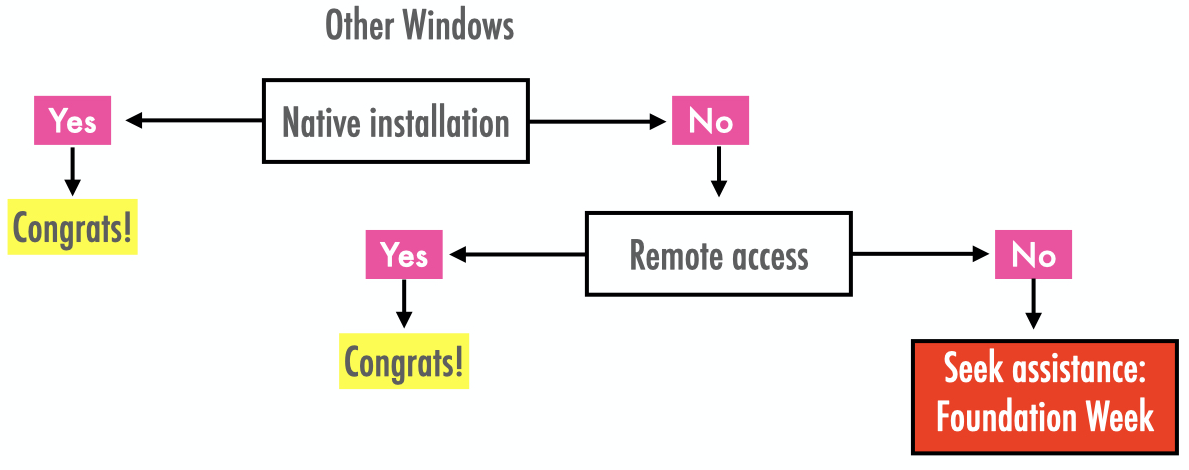
\includegraphics[width=16.51in]{figs/other_win} 

}

\caption{Decision Tree: Recommended installation for other Windows users}\label{fig:fig2}
\end{figure}

\hypertarget{mac}{%
\chapter{MacOS Installation}\label{mac}}

For each of the sections below, add:

\begin{quote}
Step-by-step instructions
\end{quote}

\begin{quote}
Insert screenshots for each step
\end{quote}

\begin{quote}
Insert a video with instructions
\end{quote}

\hypertarget{installation-via-docker}{%
\section{Installation via Docker}\label{installation-via-docker}}

\hypertarget{installing-docker}{%
\subsection{Installing Docker}\label{installing-docker}}

Draw on instructions from \href{https://gdsl-ul.github.io/the_knowledge/docker.html}{here} and \href{https://darribas.org/gds_env/guides/docker_install/}{here}

\hypertarget{installing-python}{%
\subsection{Installing Python}\label{installing-python}}

\hypertarget{running-python}{%
\subsection{Running Python}\label{running-python}}

\hypertarget{native-installation}{%
\section{Native Installation}\label{native-installation}}

Draw on \href{http://darribas.org/gds19/software.html}{A minimalist approach: conda}

\hypertarget{remote-access}{%
\section{Remote Access}\label{remote-access}}

Check with CSD

\hypertarget{linux}{%
\chapter{Linux Installation}\label{linux}}

For each of the sections below, add:

\begin{quote}
Step-by-step instructions
\end{quote}

\begin{quote}
Insert screenshots for each step
\end{quote}

\begin{quote}
Insert a video with instructions
\end{quote}

\hypertarget{installation-via-docker}{%
\section{Installation via Docker}\label{installation-via-docker}}

\hypertarget{installing-docker}{%
\subsection{Installing Docker}\label{installing-docker}}

Draw on instructions from \href{https://gdsl-ul.github.io/the_knowledge/docker.html}{here} and \href{https://darribas.org/gds_env/guides/docker_install/}{here}

\hypertarget{installing-python}{%
\subsection{Installing Python}\label{installing-python}}

\hypertarget{running-python}{%
\subsection{Running Python}\label{running-python}}

\hypertarget{native-installation}{%
\section{Native Installation}\label{native-installation}}

Draw on \href{http://darribas.org/gds19/software.html}{A minimalist approach: conda}

\hypertarget{remote-access}{%
\section{Remote Access}\label{remote-access}}

Check with CSD

\hypertarget{win10pro}{%
\chapter{Windows 10 Pro/Student Installation}\label{win10pro}}

For each of the sections below, add:

\begin{quote}
Step-by-step instructions
\end{quote}

\begin{quote}
Insert screenshots for each step
\end{quote}

\begin{quote}
Insert a video with instructions
\end{quote}

\hypertarget{installation-via-docker}{%
\section{Installation via Docker}\label{installation-via-docker}}

\hypertarget{installing-docker}{%
\subsection{Installing Docker}\label{installing-docker}}

Draw on instructions from \href{https://gdsl-ul.github.io/the_knowledge/docker.html}{here} and \href{https://darribas.org/gds_env/guides/docker_install/}{here}

\hypertarget{installing-python}{%
\subsection{Installing Python}\label{installing-python}}

\hypertarget{running-python}{%
\subsection{Running Python}\label{running-python}}

\hypertarget{native-installation}{%
\section{Native Installation}\label{native-installation}}

Draw on \href{http://darribas.org/gds19/software.html}{A minimalist approach: conda}

\hypertarget{remote-access}{%
\section{Remote Access}\label{remote-access}}

Check with CSD

\hypertarget{otherwin}{%
\chapter{Other Windows Versions Installation}\label{otherwin}}

For each of the sections below, add:

\begin{quote}
Step-by-step instructions
\end{quote}

\begin{quote}
Insert screenshots for each step
\end{quote}

\begin{quote}
Insert a video with instructions
\end{quote}

\hypertarget{installing-python}{%
\subsection{Installing Python}\label{installing-python}}

\hypertarget{running-python}{%
\subsection{Running Python}\label{running-python}}

\hypertarget{native-installation}{%
\section{Native Installation}\label{native-installation}}

Draw on \href{http://darribas.org/gds19/software.html}{A minimalist approach: conda}

\hypertarget{remote-access}{%
\section{Remote Access}\label{remote-access}}

Check with CSD

  \bibliography{book.bib,packages.bib}

\end{document}
